\documentclass[letterpaper, 11pt]{article}

\usepackage[pdftex]{graphicx}
\usepackage{epstopdf}
\DeclareGraphicsRule{*}{mps}{*}{} 

\usepackage{amsmath, amsthm, amssymb}
\usepackage{listings}
\usepackage{float}
\usepackage{enumerate}
% \usepackage{mystyle}
\usepackage{hyperref}
\usepackage{tikz}
\usepackage{fancyheadings}
\usepackage{tensor}
\usepackage{mathrsfs}
\usetikzlibrary{positioning}
\usetikzlibrary{decorations.pathmorphing}
\usetikzlibrary{arrows}
\usetikzlibrary{decorations.markings}
%\usepackage{fullpage}
\usepackage[left=0.75in, top=1.25in, right=0.75in, bottom=1.25in]{geometry}
\newcommand{\lambdabar}{{\mkern0.75mu\mathchar '26\mkern -9.75mu\lambda}}

\numberwithin{equation}{section}
\numberwithin{figure}{section}

\begin{document}

\title{Numerical Methods for Astrophysical Magnetohydrodynamics}
\author{Jim Stone}
\date{July 19, 2016}

\maketitle

\section{Lecture 1 - Astrophysical MHD}

I will mainly talk about one single class of numerical method for MHD, which is
finite volume method. Link to the \href{http://www.astro.princeton.edu/~jstone/downloads/papers/Lecture1.pdf}{slides}.

\subsection{Overview}

Why are we interested in doing numerical MHD? Most of the big questions in
astrophysics require the study of the dynamics of visible matter in the form of
plasma. For example, how do galaxies form, how do stars form, how do planets
form, etc. We are going to focus on collisionless plasma today, and for
collisional plasma additional methods are required.

The equations of inviscid ideal MHD are as follows (in units so that $\mu = 1$)
\begin{align}
  \frac{\partial\rho}{\partial t} + \nabla \cdot \left( \rho \mathbf{v} \right) &= 0 \\
  \frac{\partial(\rho \mathbf{v})}{\partial t} + \nabla \cdot \left( \rho \mathbf{v}\mathbf{v} - \mathbf{B}\mathbf{B} + P^{*} \right) &= 0 \\
  \frac{\partial E}{\partial t} + \nabla\cdot \left[ (E + P^{*})\mathbf{v} - \mathbf{B}\left( \mathbf{B}\cdot \mathbf{v} \right) \right] &= 0 \\
  \frac{\partial \mathbf{B}}{\partial t} - \nabla\times (\mathbf{v}\times \mathbf{B}) &= 0
\end{align}
where $P^{*} = P + B^2/2$ and $E = \rho v^2/2 + e + B^2/2$ are the total
pressure and total energy. The above equation is not closed, since one needs an
equation of state $P = P(\rho, T)$.

The hydro equations can be written in a compact form (in 1D)
\begin{equation}
  \label{eq:1}
  \frac{\partial \mathbf{U}}{\partial t} + \frac{\partial \mathbf{F}}{\partial x} = 0,\qquad 
\end{equation}
This is a hyperbolic system of equations. They admit wavelike solutions, in the
form of
\begin{equation}
  \label{eq:2}
  a = a_0 + a_1\exp(i\mathbf{k}\cdot \mathbf{x} - i\omega t)
\end{equation}
When $a_1\ll a_0$ waves have small amplitude, and they are in the linear regime.
When $a_1\gg a_0$ we are in nonlinear regime.

The dispersion relation for MHD waves can be found and summarized together:
\begin{equation}
  \label{eq:3}
  \left[ \omega^2 - (\mathbf{k}\cdot \mathbf{v}_A)^2 \right] \left[ \omega^4 - \omega^2k^2(v_A^2 + C^2) + k^2C^2 (\mathbf{k}\cdot \mathbf{v}_A)^2 \right] = 0
\end{equation}

The phase velocities of MHD waves can be summarized by Friedrichs diagrams.
\begin{figure}[h]
  \centering
  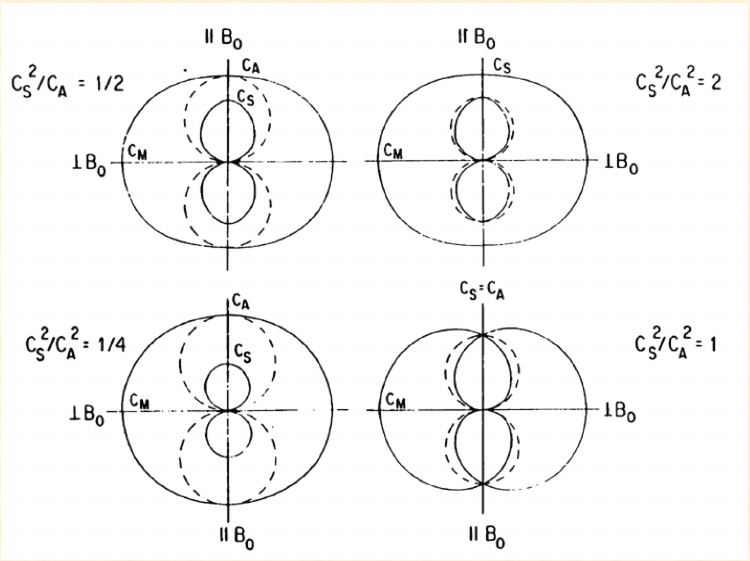
\includegraphics[width=0.8\textwidth]{Friedrichs.png}
  \caption{Friedrichs diagrams (from the slides)}
\end{figure}

However, the point of numerical simulations is to solve the full nonlinear
problem which can't be solved analytically. The simplest example is a contact
discontinuity: discontinuous change in density which constant $P$ advected at
constant $\mathbf{v}$. We can also have shocks where all variables can be
changed. In real life for example, when a plane flies across air at speed $v >
C$ it creates a shockwave. 

These kind of shocks are described by jump conditions, which are changes in
conserved variables across the discontinuity. To describe the hydrodynamic
shock, in the frame of the shock, there is a steady fluid flow toward the shock
from the upstream, and away from the show in the downstream direction. Mass,
energy and momentum are conserved in this frame. We can solve the equations for
the Rankine-Hugoniot jup conditions
\begin{equation}
  \label{eq:5}
  \frac{\rho_d}{\rho_u} = \frac{(\gamma + 1)\mathcal{M}^2}{(\gamma - 1)\mathcal{M}^2 + 2}
\end{equation}
where $M = v_u/C_u$ is the shock Mach number.

In MHD the shocks are more complicated since there are more kinds of shocks.
There can be Alfven ``shocks'' where only the transverse components of $v$ and
$B$ change discontinuously. There can be slow or fast shock, switch-on/off
shocks. These are shocks with small parameter space but very useful to test
codes to see if these can be captured.

Going beyond shocks is a zoo of linear instabilities of MHD fluids. Some of the
most important instabilities are gravitational instability, thermal instability,
Rayleigh-Taylor instability (light fluid supporting a heavy fluid under
acceleration), Richtmyer-Meshkov instability, Kelvin-Helmholtz instability (two
fluids flowing shearing across each other), and magneto-rotational instability
(in accretion disks for example). All these instabilities are important in
astrophysical conditions so we need to capture these correctly. Instabilities
often lead to turbulence, and the study of nonlinear turbulence is an important
application of the codes.

What do we mean by correctly? We need to understand what is feasible and what is
not. The dispersion relation for most MHD instabilities are unstable for a broad
range of wave numbers. However on a grid we can only have a finite resolution
depending on the grid size. Correctly means the linear growth rate of all modes
between $N\Delta x$ and $L$ are represented accurately. If we are studying
unresolved flows that is dominated by truncation error then we will get
different answer with different resolutions.

\subsection{Numerical Methods}

Lets start off by round-off error. Not all floating numbers can be represented
due to finite bit length. Rounding is correct if no machine number lies between
$x$ and its rounded value $x'$, and the difference between them is the round-off
error.

We can prove that the relative error of a rounded value is always bounded by a
small, machine dependent number
\begin{equation}
  \label{eq:6}
  \frac{|x - x'|}{|x|} < \epsilon
\end{equation}
which is the basis of all rigorous error analysis of numerical methods.

Another error is the truncation error. Numerical algorithms approximate analytic
solutions with algebraic operations. The difference between true and approximate
(numerical) solutions is the truncation error. This is under programmer control,
as oppose to the round-off error.

There are three concepts in numerical analysis that are very important:
Convergence, Consistency, and Stability. Convergence means when $\Delta x$ and
$\Delta t$ decreases, the truncation error should also decrease. Higher order
schemes often converge faster, but they cost more which puts a practical limit
on the usefulness of high order schemes. All methods are first-order for
discontinuities, so high order schemes are not very useful for shock capturing.

Consistency is another important concept which is often forgotten. It means that
the solutions of the underlying PDEs should not only converge but also converge
to the correct analytic solution. Finally stability is also important and it
means that round-off error must remain small and bounded. A solution can be
numerically unstable seeded by uncontrolled round-off error and it can grow
exponentially, which is undesirable.

The simplest discretization of a simple hyperbolic PDE is the forward-time
centered-space (FTCS) finite differencing method.
\begin{equation}
  \label{eq:7}
  \frac{\partial u}{\partial t} + a\frac{\partial u}{\partial x} = 0,\Longrightarrow \frac{u_j^{n+1} - u_j^n}{\Delta t} + a \left( \frac{u_{j+1}^n - u_{j-1}^n}{2\Delta x} \right) = 0
\end{equation}
We can perform a von Neumann stability analysis to show that this method is
unconditionally unstable. To show this we can insert
\begin{equation}
  \label{eq:8}
  u_j^n = \xi^n\exp(ikj\Delta x)
\end{equation}
When we substitute this into the finite difference equation we get $\xi(k) = 1 -
i(a\Delta t/\Delta x)\sin k\Delta x$. The amplitude of $\xi(k) > 0$ for all
$\Delta t > 0$. Therefore the method will blow up for any evolution in time.

However this is easy to fix by changing the time derivative to use an average of
$u$ at $t^n$ (Lax-Friedrichs):
\begin{equation}
  \label{eq:9}
  \frac{u_j^{n+1} + (u_{j+1}^n + u_{j-1}^n)/2}{\Delta t} + a \left( \frac{u_{j+1}^n - u_{j-1}^n}{2\Delta x} \right) = 0
\end{equation}
Now if we do the same analysis then we see $\xi(k) < 1$ iff
\begin{equation}
  \label{eq:10}
  \frac{a \Delta t}{\Delta x} \leq 1
\end{equation}
which is known as the Courant-Levy-Friedrichs (CFL) stability criterion.

Why does this work? In fact this LF equation introduces explicit numerical
viscosity which makes the algorithm stable, since we can rewrite the finite
difference equation to be %TODO

However the LF method has huge diffusion, so not recommended for practical use
nowadays. Another way is to use the Upwind methods
\begin{equation}
  \label{eq:11}
  \begin{split}
  \frac{u_j^{n+1} - u_j^n}{\Delta t} =&
    -a \left( \frac{u_j^n - u_{j-1}^n}{\Delta x} \right), \quad \text{if }a > 0 \\
    &-a \left( \frac{u_{j+1}^n - u_j^n}{\Delta x} \right), \quad \text{if }a < 0
  \end{split}
\end{equation}
This method has less diffusion than LF.

Both the above methods are diffusion methods. They add diffusion error to the
result, such that a localized perturbation will tend to diffuse away. Some other
methods (e.g. LW) will add dispersion error (with different dispersion
relation). Diffusion errors are acceptable, but dispersion errors will be
disastrous in some situations and should be avoided at all cost.

\subsection{Finite Volume Methods}

There is a zoo of algorithms for MHD. To list some of them: Finite-differencing
with hyper-viscosity, operator split methods, finite-volume methods, spectral
methods, discontinuous Galerkin methods, MHD SPH methods.

Finite volume MHD codes are popular and there are a variety of them: Athena,
VAC, AstroBEAR, PLUTO, FLASH, HARM, Enzo, Cosmo++, etc. This lecture will focus
on the methods in Athena.

\subsubsection{Discretization}

How does finite volume discretization work? We first discretize the space
$\mathbf{x} \rightarrow (x_i, y_i, z_i)$. We discretize time into $t \rightarrow
t^n$. We discretize continuous variables to be volume average values for each
cell. This is an important facet of the scheme, since it is not a sampling, but
an averaging.

We use a staggered mesh where scalars are cell-centered and magnetic fields are
defined at cell faces. Cell-centered quantities are volume-averaged and face
centered quantities are area-averaged. Since we mostly compute the curl of $B$,
area averaging is the natural discretization of the magnetic field.

We write the conservation laws in the form of hyperbolic equations
\begin{equation}
  \label{eq:12}
  \frac{\partial \mathbf{U}}{\partial t} + \frac{\partial \mathbf{F}}{\partial x} + \frac{\partial \mathbf{G}}{\partial y} + \frac{\partial \mathbf{H}}{\partial z} = 0
\end{equation}
We can integrate the equation over the volume of a grid cell, and over a
timestep $dt$, we can get an exact finite difference equation, where the
differences are differences over average values.

For the induction equation we use the finite area discretization, which is a
similar concept, but averaging over an area instead of a volume, which is
natural for the equation. Again we obtain an exact equation.

To summarize, mass, momentum, and energy fields are cell-centered. Fluxes are
face centered, and EMFs are edge-centered. The key is now to compute these
fluxes and EMFs all at once!

\subsubsection{Godunov Method}

The answer is to use Godunov's method. Difference in cell-averaged values at
each grid interface define a set of Riemann problems (evolution of initially
discontinuous states). The solution of Riemann problems averaged over cell gives
time evolution of cell-averaged values, until the wave hits the grid interfaces.
Due to conservation we don't even need to solve the Riemann problem exactly. We
only need to compute the flux through the interfaces between the cells, so we
only need to solve the Riemann problem at every cell interface.

So we introduce a Riemann solver. There are many possible solvers. In MHD
nonlinear Riemann solvers are complex because of the many families of waves and
many characteristics. In addition, the equations of MHD are not strictly
hyperbolic. Therefore MHD Gudonov schemes use approximate or linear Riemann
solvers.

There is Roe's method which keeps all 7 characteristics but treat each as a
simple wave. There is HLLE method which keeps only the largest and smallest
characteristics, but averages intermediate states in-between. There is also the
HLLC method which adds entropy and Alfven waves back into the HLLE method giving
2(4) intermediate states.

To determine which Riemann solver is the best, one needs to explore the use of
each. However the use of a Riemann solver is a benefit, not a weakness, since it
makes shock capturing more accurate: we encode in the numerical scheme a inherit
way of dealing with discontinuities.

We can use higher order methods to define Riemann problems to reconstruct
left-right states within cells using piecewise linear/parabolic methods. If we
need to do multidimensions, typically one split the equations directionally. One
solve the equations in $x$ directions first, then do it for $y$ with results
from the $x$ update, and so on. However in MHD this kind of splitting will not
preserve $\nabla\cdot \mathbf{B} = 0$. One needs to use directionally unsplit
methods. One first computes first order fluxes at every interface, use these
fluxes to advance solution for $\Delta t/2$, compute L/R states using this
time-advanced state, and fluxes, and then finally advance solutions over a full
timestep using the new fluxes.

\subsubsection{Constraints and Tests}

We also need to specify boundary conditions. Most codes apply boundary
conditions using ghost/guard cells.

How do we keep $\nabla\cdot \mathbf{B} = 0$? There are many ways. One way is to
do nothing and assume everything is okay. One way is to evolve $B$ using vector
potential $\mathbf{A}$, but this requires second derivatives which can be
numerically dangerous. One way is to remove solenoidal part of $\mathbf{B}$
using flux-cleaning, by setting $\mathbf{B} \to \mathbf{B} - \nabla\phi$ and
solving an elliptic PDE at every time step. Finally the way used in Athena is to
evolve the integral form of induction equation with Constrained Transport so
that $\nabla\cdot \mathbf{B} = 0$ is automatically conserved.

However the last CT method requires $E$ field at grid cell centers while they
are defined on edges. Arithmetic averaging destroys the scheme so we need an
algorithm to reconstruct $E$ field at the corner.

For stability we have to observe the CFL condition
\begin{equation}
  \label{eq:13}
  \Delta t \leq \frac{\Delta t}{v + C}
\end{equation}
We define the Courant number $C$ to be the ratio between lhs and rhs. For
stability we need $C<1$, and for multidimensions we usually need $C <
1/N_\text{dim}$.

There are many ways to test correctness. One simple way is to test linear wave
convergence in 3D. We measure the RMS error in $\mathbf{u}$ after propagating
a pure eigenmode for one wavelength. The error better decrease linearly with
increasing resolution. Some other tests include nonlinear circularly polarized
Alfven waves, shocktubes, MHD instabilities, etc.





\end{document}
